% !TeX root = ../Bachelorarbeit.tex
\chapter{Anhang - Informationen zu Tools}
\label{cha:Anhang_Info}

\section{Erweiterungen von Visual Studio Code}
\label{sec:extensions}
Die installierten Erweiterungen des Editors Visual Studio Code werden folgend alphabetisch aufgelistet: 
\begin{multicols}{2}
	\begin{itemize}
		\item alefragnani.project-manager
		\item austin.code-gnu-global
		\item christian-kohler.path-intellisense
		\item dbaeumer.vscode-eslint
		\item donjayamanne.githistory
		\item eamodio.gitlens
		\item eg2.tslint
		\item formulahendry.code-runner
		\item James-Yu.latex-workshop
		\item mitaki28.vscode-clang	
	\end{itemize}
	\columnbreak
	\begin{itemize}
		\item ms-vscode.azure-account
		\item ms-vscode.cpptools
		\item ms-vscode.csharp
		\item msjsdiag.debugger-for-chrome
		\item redhat.java
		\item robertohuertasm.vscode-icons
		\item rokoroku.vscode-theme-darcula
		\item streetsidesoftware.code-spell-checker
		\item streetsidesoftware.code-spell-checker-german
		\item WallabyJs.wallaby-vscode
		\item zhuangtongfa.Material-theme
	\end{itemize}
\end{multicols}

\section{Ordnerstruktur der CD}
\label{sec:treeCD}

\begin{figure}[htp]
	\centering
	\captionsetup{justification=centering}
	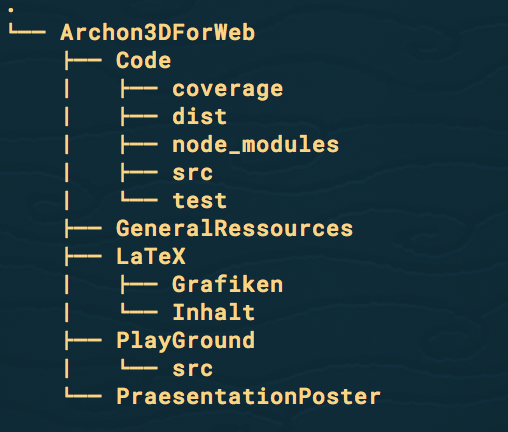
\includegraphics[width=0.45\textwidth]{TreeCD}
	\caption[Ordnerstruktur CD]{Ordnerstruktur der CD}
	\label{fig:TreeCD}
\end{figure}